%!TEX root = ../neo4j.tex

\section{Introduction}
Neo4j is a transactional and graph based database. It was first released in 2010. Neo4j is written in Java and available under two different licences. 


\subsection{Neo4j DB}
Neo4j has its own query language which is called Cypher. Cypher concentrates on pattern search. It is similar to SQL, both are descriptive languages. Cypher can be used in the command line, but all properties about transaction behaviour are also valid for transactions executed by a terminal or a program. \nocite{neo4jman:2011}\\
Queries are run in a transaction. Either there exists already a transaction or one is created. It is possible to commit several queries to one transaction. "A transaction will either fully succeed, or not succeed at all" \cite{}. Changes of a query are held in memory until the hole query has finished executing. This needs a lot of heap space and therefore it is important to structure queries. Neo4j supports the ACID properties - atomicity, consistency, isolation and durability. In case of a failure of a transaction a roll back is done. Neo4j offers several options for managing locking of resources. On the one hand there is a default locking behaviour, on the other hand tools are given to archive a higher level of isolation for transactions. Additionally, it uses deadlock detection algorithms.\\
Neo4j databases are accessible via a Java API and therefore can be embedded in Java applications. It also supports batch processing for large amounts of data.

\subsection{Example}
As an example we modelled  the relation between books, authors and publishers. Authors write books and publishers publish books. To start working with the database, Neo4j has to be run from the command line or terminal. After the server did start, a graphical user interface can be accessed through a browser. This graphical user interface has its own command line in which Cypher statements are executed.\\
Figure \ref{example-graph} shows how our example looks in Neo4j. This picture is given by Neo4j in the browser view.

\begin{figure}
	\centering
		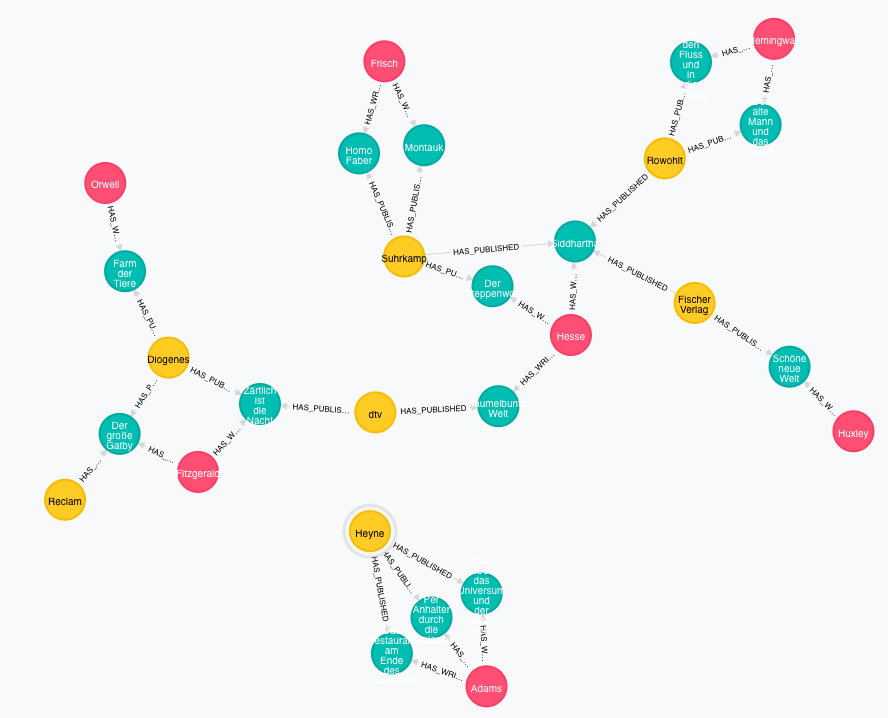
\includegraphics[width=\linewidth]{images/Neo4j_Graph.png}
	\caption{Example Graph}
	\label{example-graph}
\end{figure}

\subsection{Queries}
Neo4j offers a lot of possibilities for queries. In this section, some query examples are given in Cypher syntax for the example graph.\\
The syntax of Cypher statements are similar to SQL statements. Listing \ref{Cypher-Syntax} shows the basic structure  of a statement.
 
\begin{lstlisting}[language={Cypher}, caption={Cypher Syntax}, label={Cypher-Syntax}]
MATCH <pattern> WHERE <conditions> RETURN <expressions>
\end{lstlisting}

\paragraph{CREATE}
The CREATE statement can be used to create new nodes as well as create relations between notes. Listing \ref{create_node} shows how to create the author Fitzgerald. The CREATE statement is started with parenthesis to indicate a node. The first information given to the CREATE statement is the ID of the node, followed by a colon and a lable given to the node. In this case the ID is fscottfitzgerald and the label for the node is Author. All properties follow in braces. The node here has three attributes: name, first-name and stage-name.

\begin{lstlisting}[language={Cypher}, caption={Create Node}, label={create_node}]
CREATE (fScottFitzgerald:Author { name : 'Fitzgerald', firstname : 'Francis Scott Key', stagename : 'F. Scott Fitzgerald'})
\end{lstlisting}

The statement for creation of a relation looks a bit different. Listing \ref{create_relation} shows an example where the relation between Fitzgerald and his book is made. The node ID from which the relations starts is put in parenthesis at the beginning. Then the kind of relation is defined with brackets. Beginning with a colon the relationship type is defined, followed by all properties in braces. After the relationship information are finished an arrow points to the end node, again defined by the node ID in parenthesis. To use the ID to identify a node is only possible if the node is created in the same transaction as the relation. Otherwise the node has to be found via the MATCH statement. On the other hand, if one ore two nodes do not exist when create relation statement is executed, this nodes will be created automatically. 

\begin{lstlisting}[language={Cypher}, caption={Create Relation}, label={create_relation}]
CREATE (fScottFitzgerald)-[:HAS_WRITTEN { year : '1925'}]->(derGrosseGatsby)
\end{lstlisting}

\paragraph{MATCH}
MATCH is used to find nodes. The simplest MATCH statement is shown in listing \ref{simple_match}. This statement returns everything in the graph. E.G. this statement was used to extract figure \ref{example-graph}, an image of the graph which is shown above. Furthermore it is used for nearly every operation in the graph. One can find nodes of a special type, nodes or relations with a certain property or just certain information. If an item is found the statement can be extended, e.g. to add a CREATE statement or add a new property. Listing \ref{relation_match} is an examples which shows how to create a new relation between two existing nodes. This statement sets Heyne as the publisher of Homo Faber.

\begin{lstlisting}[language={Cypher}, caption={Simplest Match Statement}, label={simple_match}]
MATCH n RETURN n
\end{lstlisting}

\begin{lstlisting}[language={Cypher}, caption={Match and Create Relation}, label={relation_match}]
MATCH (bb:Book), (vv:Publisher) WHERE bb.title = "Homo Faber" AND vv.name = "Heyne" CREATE (vv)-[r:HAS_PUBLISHED]->(bb) RETURN r
\end{lstlisting}

Neo4j offers the possibility to solve a graph. It provides statements to find the shortest path through a graph (also possible for sub-graphs) or select the surrounding of a node with a certain radius. These statements are on the basis of the MATCH statement too.

\paragraph{DELETE}
In Neo4j it is only possible to delete the graph. This means, all nodes and relations are deleted, but all labels will remain. These can only be delete if the whole database is deleted. The DELETE statement also uses the MATCH statement as a basis. First, all nodes and all relations of these nodes are selected. It is important that a node which is to be deleted has no relations any more. It is not necessary to first to delete all relations and divide the operation in two transactions. With OPTIONAL MATCH this is done automatically by Neo4j. The DELETE statement takes every selected item and deletes it.

\begin{lstlisting}[language={Cypher}, caption={Delete Graph}, label={delete}]
MATCH (vv:Publisher), (aa:Author), (bb:Book) OPTIONAL MATCH (vv)-[hp]-(), (aa)-[hw]-() DELETE aa, vv, bb, hp, hw
\end{lstlisting}